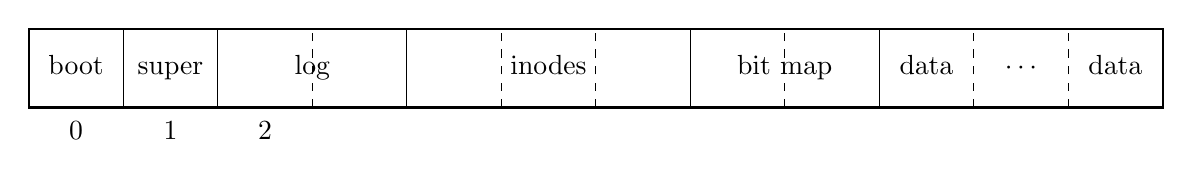
\begin{tikzpicture}[x=1.2cm,y=1cm]

  % One x-unit = one disk block (all blocks the same width).
  % 12 equal blocks: boot super | log(2) | inodes(3) | bit map(2) | data ... data
  \draw[thick] (0,0) rectangle (12,1);

  % Solid dividers between sections
  \foreach \x in {1,2,4,7,9}
    \draw (\x,0) -- (\x,1);

  % Dashed dividers between blocks within a multi-block section
  \foreach \x in {3,5,6,8,10,11}
    \draw[dashed] (\x,0) -- (\x,1);

  % Section labels, centered over each section and sharing a common baseline
  \tikzset{seclabel/.style={anchor=base}}
  \node[seclabel] at (0.5,0.42)  {boot};
  \node[seclabel] at (1.5,0.42)  {super};
  \node[seclabel] at (3,0.42)    {log};
  \node[seclabel] at (5.5,0.42)  {inodes};
  \node[seclabel] at (8,0.42)    {bit map};
  \node[seclabel] at (9.5,0.42)  {data};
  \node          at (10.5,0.5)   {$\cdots$};
  \node[seclabel] at (11.5,0.42) {data};

  % Block numbers below the first three blocks
  \node[below] at (0.5,-0.05) {0};
  \node[below] at (1.5,-0.05) {1};
  \node[below] at (2.5,-0.05) {2};

\end{tikzpicture}
